\documentclass[review]{elsarticle}

\usepackage{lineno,hyperref}
\modulolinenumbers[5]
\usepackage{booktabs}
\usepackage{graphicx}
\usepackage{float}
\graphicspath{ {./images/} }
\usepackage{adjustbox}

\usepackage{threeparttable}
\usepackage{amsmath}
\usepackage[font=small,skip=0pt]{caption}

\journal{International Journal of Forecasting}

%%%%%%%%%%%%%%%%%%%%%%%
%% Elsevier bibliography styles
%%%%%%%%%%%%%%%%%%%%%%%
%% To change the style, put a % in front of the second line of the current style and
%% remove the % from the second line of the style you would like to use.
%%%%%%%%%%%%%%%%%%%%%%%

%% Numbered
%\bibliographystyle{model1-num-names}

%% Numbered without titles
%\bibliographystyle{model1a-num-names}

%% Harvard
%\bibliographystyle{model2-names.bst}\biboptions{authoryear}

%% Vancouver numbered
%\usepackage{numcompress}\bibliographystyle{model3-num-names}

%% Vancouver name/year
%\usepackage{numcompress}\bibliographystyle{model4-names}\biboptions{authoryear}

%% APA style
%\bibliographystyle{model5-names}\biboptions{authoryear}

%% AMA style
%\usepackage{numcompress}\bibliographystyle{model6-num-names}

%% `Elsevier LaTeX' style
\bibliographystyle{elsarticle-num}
%%%%%%%%%%%%%%%%%%%%%%%

\begin{document}

  \begin{frontmatter}

    \title{A novel interval electricity price forecasting using Residual Neural Networks (ResNet)}
    % \tnotetext[mytitlenote]{Fully documented templates are available in the elsarticle package on \href{http://www.ctan.org/tex-archive/macros/latex/contrib/elsarticle}{CTAN}.}

    %% Group authors per affiliation:
    % \author{Pornchai Chaweewat\fnref{myfootnote}}
    \author{Pornchai Chaweewat\fnref{myfootnote}}
    \author{J G singh\fnref{myfootnote2}}

    \address{Department of Energy, Environmental and Climate Change, School of Environmental, Resource and Development, Asian Institute of Thechnology, Thailand}
    \fntext[myfootnote]{email: chaweewat.p@gmail.com}
    \fntext[myfootnote2]{email: jgsingj@ait.ac.th}

    % %% or include affiliations in footnotes:
    % \author[mymainaddress,mysecondaryaddress]{Elsevier Inc}
    % \ead[url]{www.elsevier.com}
    %
    % \author[mysecondaryaddress]{Global Customer Service\corref{mycorrespondingauthor}}
    % \cortext[mycorrespondingauthor]{Corresponding author}
    % \ead{support@elsevier.com}
    %
    % \address[mymainaddress]{1600 John F Kennedy Boulevard, Philadelphia}
    % \address[mysecondaryaddress]{360 Park Avenue South, New York}

    \begin{abstract}
      This paper proposed a novel electricity price forecasting method based on a novel Residual Neural Network (ResNet) for probabilistic electricity price forecasting under spike price environment.
      The modern electricity price became more fluctuated and generally unanticipated spike price.
      The use of prediction interval or probabilistic forecasting was interested due to it help market participants to submit effective bids with low risks.
      A proposed new model was developed from ResNet approach which it capable of spike price and interval price value prediction.
      The proposed ResNet was consisting of two network layers.
      First neural network layers was spike prediction.
      The output of second neural network layers formulated interval price forecasting by two methods; quantile regression and mean and varience estimation method.
      The proposed forecasting models was demonstrated with GEFCom2014 dataset.
      The dataset is consisting of 15 tasks for electricity price forecasting where high and spike price are included.
      The results were compared with benchmarks as provided by GEFCom2014, Quantile Regression Average (QRA) and multilayer perceptron network (MLP) approaches.
      The performances of forecasting models were evaluated in term of accuracy and reliablity metrics by Pinball Loss Function and Coverage Width-based Criterion (CWC), respectively.
      The significant outcome of this paper was that forecasting model cooperated with spike price prediction imporved the forecasting's performance in term of accuracy and reliability aspects.
      Moreover, increasing in confidence level of ResNet models could generates lower CWC values and represent high reliability's satification.
    \end{abstract}

    \begin{keyword}
      GEFCom2014, interval forecasting, quantile regression, mean and varience estimation
    \end{keyword}

  \end{frontmatter}

  \linenumbers

  \section{Introduction}

    Since the transformation of the deregulation of modern power systems, electricty price forecasting has become more important process to energy market's participants at planning and operation levels.
    As a result of higher number of fluctuated electricity price as well as the number of the spike price occurences.
    The occurrences of spike price can cause financial damage to both customers and producers.
    The spike prices can be reach several times to thousand times of the normal price.
    Spike price appears due to increasing intermittent electricity production makes electricity prices more volatile, with spikes appearing either as very high prices (due to sudden lack of available generation) or as negative prices (due to excess of renewable generation).
    Several evidences shows that the spike prices are around 100$\$$/MWhr may simply resulted from normal congestion or unexpected overload, while spike price around $\$$500/MWhr led by lacking of reserve.
    This case the day ahead clearing price was the dominant feature what indicate insufficient reserve. The spike price aboved $\$$1,000/MWhr should be the consequence of the outage or breakdown of the generation or transmission system.
    Such outage or breakdown many could came from many factors, like weather, load profile, etc  \cite{He2016}.
    \cite{SINGHAL2011550} provided fundamental reasons of spike price which are volatility of fuel price, load uncertainty, fluctuation in hydroelectricity production, generation outage, transmission congestion, behavior of market participation and market manipulation.
    \cite{GONZALEZSOTRES2017338} studied on technique and economical of on centralized voltage control with high PV penetration in Portuguese network.
    These results illustrated that improvement in both forecasting tools and communication systems have significant impact on dedicate resources and voltage control.

    % (talk about point of forecating, 1 method, 2 measurement, 3 problems)
    Over the past few decades, many powerful forecasting algorithms have been developed (for a recent comprehensive review, see \cite{Weron2014}).
    The majority of emprical studies was on point forecasting (or call expected value of the spot price).

    % (mention about problems of poing of forecasting, introduct to interval forecasting)
    The conventional point predictions produced no information about the sampling erros and the predicition accuracy.
    This lead to confidence intervals (CIs) and prediction intervals (PIs).
    CIs and PIs were two well-know toosl for quantifying and representing the uncertainty of predicitons.
    In literature, several methods have been proposed for construction of PIs and CIs assessment.
    Lower Upper Bounds Estimation (LUBE) method were formulated using mean and varience estimation which was proposed in \cite{Khosravi2011}.
    In addition, delta technique for PI construction was presented in \cite{KhosraviA2010}.

    % (mention on used of deep residual neural network and why we use this method)
    In computaional intelligent area, Residual neural network (ResNet) was widely used in computer vision and pattern reconigtion \cite{DBLP:journals/corr/HeZRS15}, \cite{DBLP:journals/corr/ZagoruykoK16}.
    ResNet was modified from deep Feed Forward Neural Networks (FFNNs) with extra connections (or called skip connections), passing input from one layer to a late layer as well as the next layer as shown in Figure~\ref{Fig:Basic_DRNN}.
    However, there were no used of ResNet in forecasting applications.

    \begin{figure}[H]
      \centering
      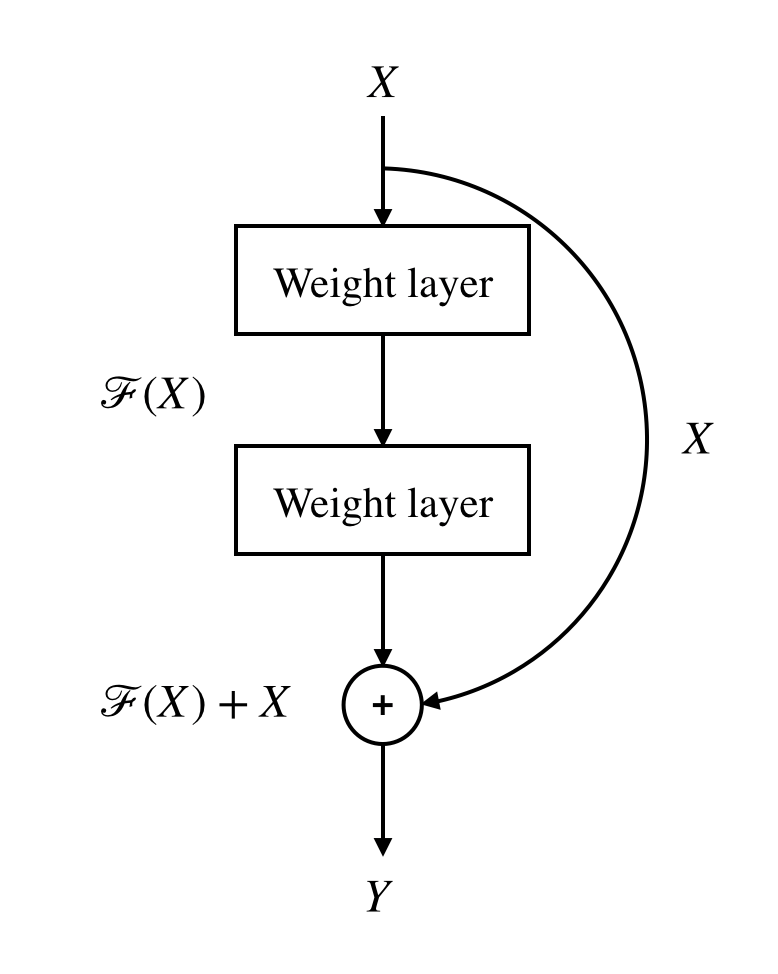
\includegraphics[width=5cm]{basic_DRNN}
      \caption{Basis concept of Residual Neural Network (ResNet)}
      \label{Fig:Basic_DRNN}
    \end{figure}


    % (proposal)
    Therefore, this paper seek to apply ResNet in electricity price forecasting.
    The performance results of the ResNet forecasting model were also compared with linear regression and MLP techniques.

    The novelty of this study is twofold.
    First, ResNet is first used in field of electricty price forecasting. Using this approach, the probabilistic electricity price forecasting can sastified both accuracy and reliability aspects.
    Second, CWC are used to evalueate interval electricity price forecasting.

    % The novelty of this study is threefold.
    % First, customer behaviors are integrated into the framework.
    % Each customer is handled individually, and the work shift constraint is considered.
    % Second, a game-theoretic approach to simulate the interaction between the utility and customers is proposed.
    % Using this approach, both optimal TOU pricing and demand response can be achieved simultaneously in the Nash-equilibrium, and the conflicting economic interests of the utility and customers can be captured clearly.
    % Third, different kinds of scenarios are investigated in case studies, which indicate that profitable results can be achieved for both sides and provide meaningful managerial insights for the practi- tioners.
    % The main findings in this study are summarized as follows.
    % (i) A good TOU price can be obtained by the game-theoretic model with the consideration of customer behaviors to create a win-win situation for the utility and customers.
    % (ii) The utility can control the interrelationship between two sides to improve its own profit. Meanwhile, attentions must be paid to the customer's credibility.
    % (iii) The customers are segregated naturally when facing the opportunity of TOU program. Therefore, the utility only need focus on the customer with a small penalty factor and a large auxiliary coefficient.
    % In fact, a small portion of customers joining the TOU program can also lead to a large improvement in utility's profit.
    % (iv) The profit of utility from the launch of TOU program is mainly affected by the expected values ofthe parameters on the client side, while it

    % (structure)
    The remainder of the paper is organized as follows.
    First, the problem formulation is presented in brief in section 2.
    The, the main features of the ANN algorithm are presented.
    Next, the results after prediction in different cases of proposed method  are discussed in section 3.
    Finally, conclusions are drawn in the last section of this paper.

  \section{Problem formulation}
    This section will descript construction of two proposed forecasting models; Multilayer Percepton (MLP) and Residual Neural Network (ResNet) model.
    The MPL model will represent electricity price forecasting without spike price prediction (see related work in \cite{Dudek2016}) and the ResNet model will represent electricity price forecasting with spike price prediction within the model.
    Both model will generate upper and lower bounds with respect to given confidence levels (5$\%$, 10$\%$, 15$\%$, 20$\%$, and 25$\%$).
    The upper and lower bound will generate using quantile regression and mean and varience estimation metod.

    \subsection{Proposed ResNet on interval price forecasting}
      Here is description of structure of a proposed ResNet for interval electricity price forecasting.
      As mention eariler, ResNet is constructed with plain layers and skip connections or called 'short-cut' to jump over some layers.
      The plain layers in this study consisted of probability spike price layers and price value layers.
      Firure~\ref{Fig:proposed_ResNet} illustrates a proposed novel ResNet for interval electricity price forecasting.
      \begin{figure}[H]
        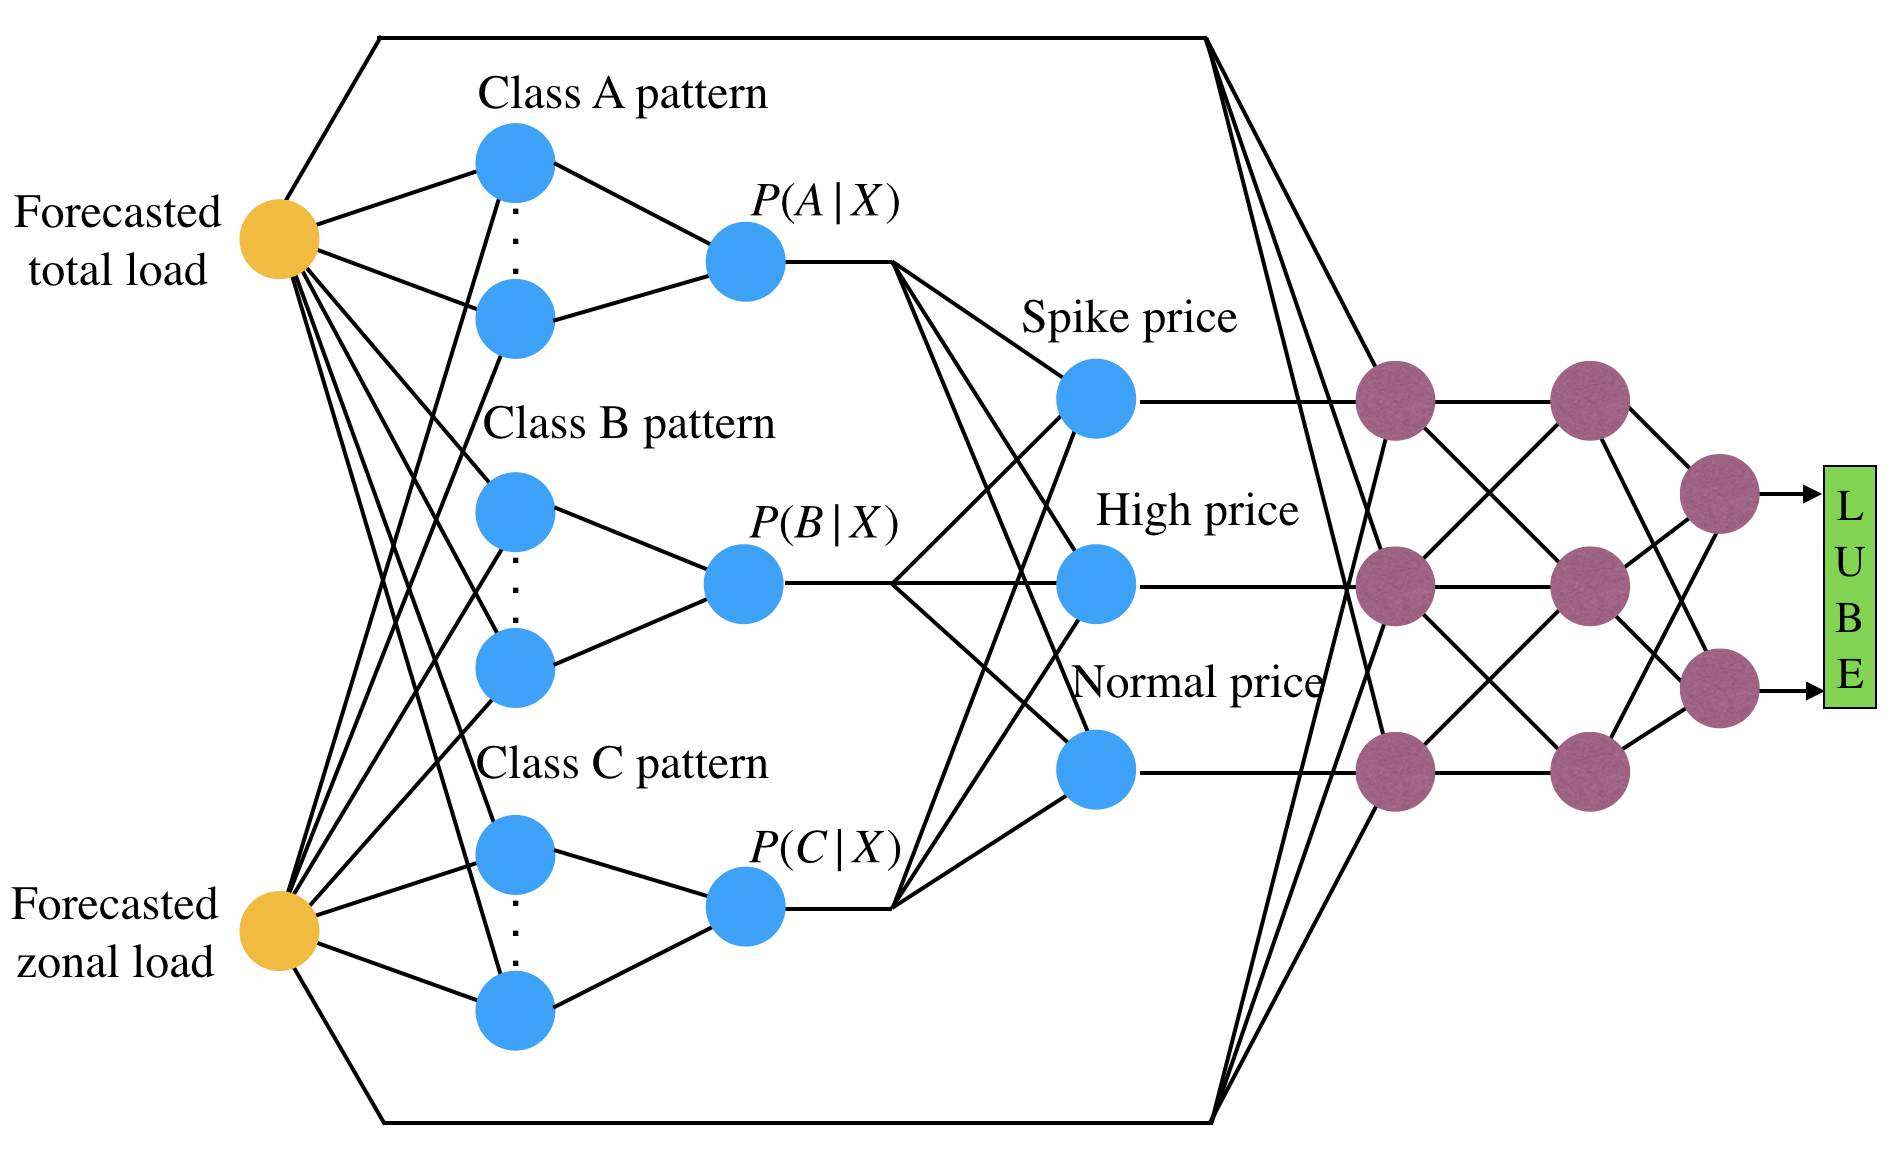
\includegraphics[width=12cm]{proposed_PDRNN}
        \caption{A proposed novel ResNet for interval electricty price forecasting application.}
        \label{Fig:proposed_ResNet}
        \centering
      \end{figure}
      The input data, forecasted system load and forecasted zonal load data , are fed to probabilistic spike price layer and price value layer.
      The output of probability spike price layer is normal, high and spike price probabilistic value $P(A)$, $P(B)$, $P(C)$.
      Then, it multiplies with fed input value to become inputs of price value layers.
      The result of the ResNet is two values of forecasted upper and lower bound ($U_{t}$, $L_{t}$)of electricty price at hour $t$ which will be descript in next section.

      In brief, the proposed ResNet consist of two network leyers.
      First is classification layer of normal, high and spike price probability.
      Second is regression layer to produce electricity  forecasting value.
      The input data is fed to second layers through short-cut paths.

    \subsection{The lower upper bound estimation}
      The lower upper bound estimation (LUBE) of interval electricity price forecasting are formulated using two methods; quantile regression, and mean and varianece estimation, respectively.
      Firstly, QR method represents asymmetrical LUBE with relation with confidence level ($\alpha$) value from quantile function as express in Equation~\ref{eq.QR}.
      \begin{equation}
        [L_{i}, U_{i}]=
        \begin{cases}
        L_{i}=\int_{0}^{a} ppf(x) dx\\
        U_{i}=\int_{1-a}^{1} ppf(x) dx
        \end{cases}
        \label{eq.QR}
      \end{equation}
      The $L_{i}$ and $U_{i}$ are lower and upper bounds generated from quantile function $\int ppf(x) dx$ with given input $x$.

      Secondaly, MV method represents symmetrical LUBE with relation with confidence level ($\alpha$) value from normal distribution function as express in Equation~\ref{eq.MV}.
      \begin{equation}
        [L_{i}, U_{i}]=
        \begin{cases}
          L_{i}=\bar{x} - z_{\alpha} \times \sqrt{\hat{\sigma}^2}\\
          U_{i}=\bar{x} + z_{\alpha} \times \sqrt{\hat{\sigma}^2}
        \end{cases}
        \label{eq.MV}
      \end{equation}
      where $\bar{x}$ and $\hat{\sigma}^2$ is mean and variance values generated from proposed forecasting model. $z_{\alpha}$ is critical value at confidence level $\alpha$.
      Figure~\ref{Fig:UB_LB_MV_PDRNN} illustrates brief proposed interval electricity price forecasting model based on ResNet with quantile regression and mean and varience method or called ResNet-QR and ResNet-MV.
      \begin{figure}[H]
        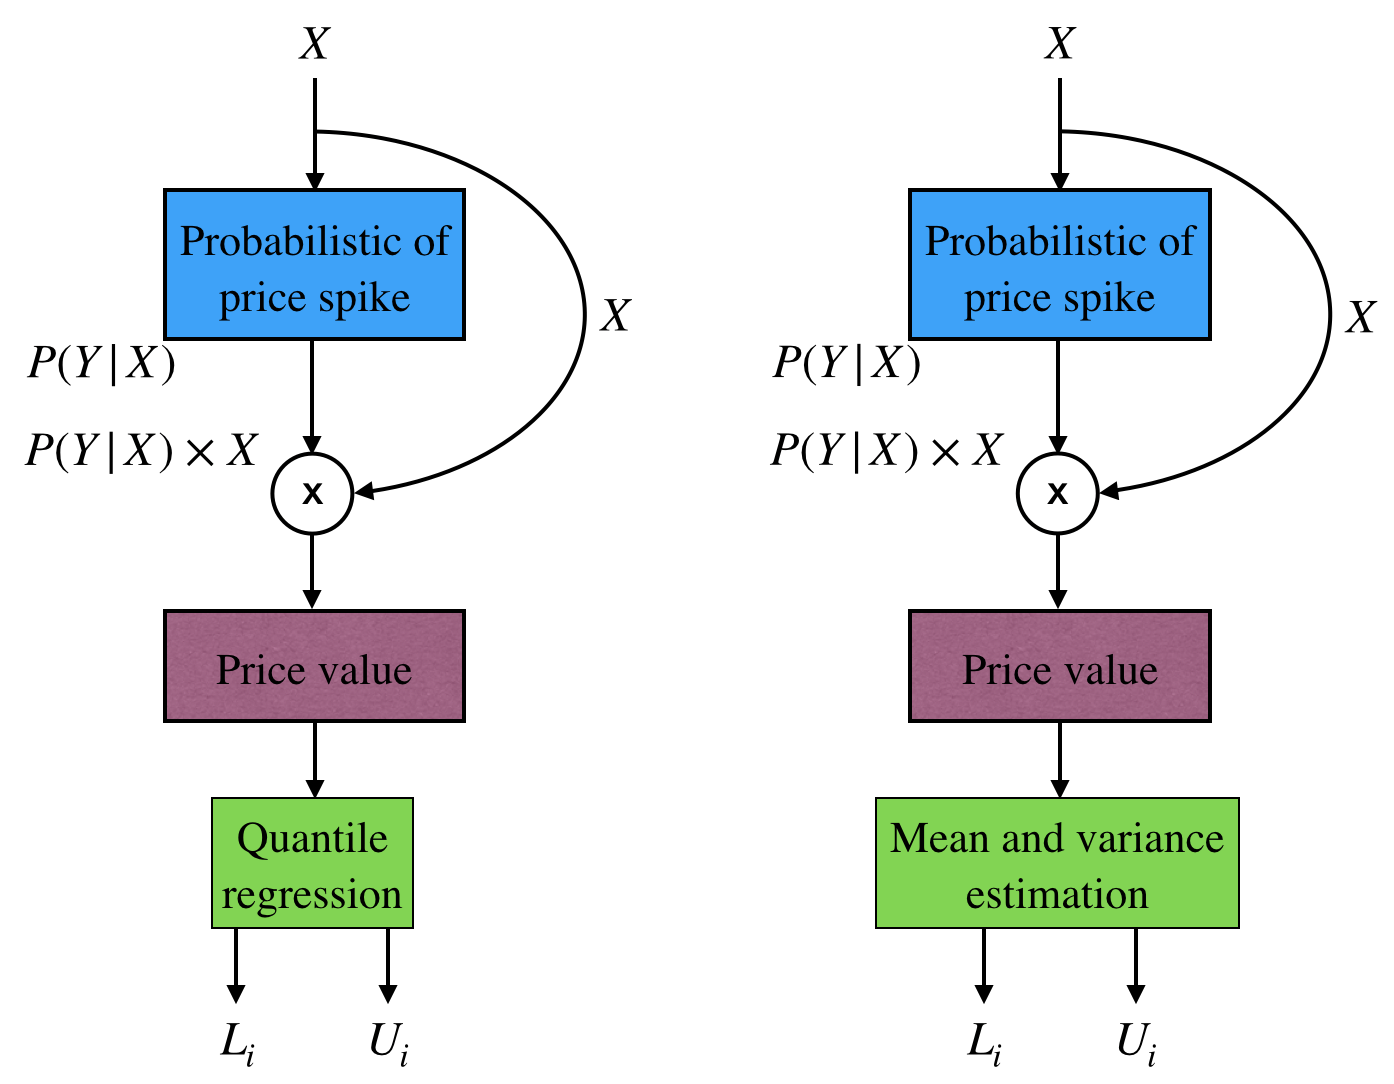
\includegraphics[width=12cm]{UB_LB_MV_PDRNN}
        \caption{The proposed ResNet models with LUBE (left) quantile regression and (right) mean and variance estimation.}
        \label{Fig:UB_LB_MV_PDRNN}
        \centering
      \end{figure}
      In Figure~\ref{Fig:UB_LB_MV_PDRNN}, the proposed ResNet-QR and ResNet-MV model consist of two main block; price spike prediction and price value estimation. $X$ are load value set. In this paper, GEFCom2014 provides total zonal load and total system load. $F()$

    \subsection{Evaluation metrics}
      This section will descript evaluation metrics on accuracy and reliable point of view.
      In term of accuracy aspect, the forecasting results will be analysed using pinball loss function.
      The Coverage Width-based Criterion (CWC) will take care of reliability aspect.

      \subsubsection{Accuracy aspect}
        The widely used measurement of forecasting's accuracy is mean absoulute error (MAE) which is simply and generalized method.
        MAE work well of point of forecasting (single value).
        However, this problem is to formulate upper and lower bound of forecasting which is cooperated with confidence value.
        Hence, general MAE is not satisfied in this case.
        Pinball loss function are proposed in \cite{Maciejowska2016}, also be benchmark of this paper, which returns the values or called loss values that can be interpreted as accuracy of mean-varience and quantile regression forecasting models.
        The pinball loss function is formulated in Equation~\ref{eq.pinball}.

        \begin{equation}
          L_{\tau}(y,z) =
          \begin{cases}
            (y-z)\tau & \text{if  $y>=z$} \\
            (z-y)(1-\tau) & \text{if  $z>y$}
          \end{cases}
          \label{eq.pinball}
        \end{equation}
        where $L_{\tau}(y,z)$ is pinball loss function at $\tau$ confidence level, $y$ is forecasted electricity price and $z$ is actual electricty price.
        The final score of pinball loss function was computed as average $L_{\tau}$ across 24 hours for each task.
        The $\tau$ in this paper is 0.05, 0.10, 0.15, 0.20 and 0.25 which are represent 5$\%$, 10$\%$, 15$\%$, 20$\%$ and 25$\%$ confidence levels.
        The important results of pinball loss function is that the lower pinball loss, the more accurate forecasting model.

      \subsubsection{Reliability aspect}
        In term of reliability measurement, the performances of forecasting model are measured to ensure that the ranges of interval electricity price forecasting can cover the observation values both quality and quantity.

        First,  PI converage probility (PICP) refers to the ability of the constructed PIs to capture the actual target variables.
        PICP can be methematically stated as
        \begin{equation}
          \text{PICP} = \frac{1}{N} \sum_{i=1}^{N} C_{i}
          \label{eq.PICP}
        \end{equation}
        where
        \begin{equation}
          C_{i} =
          \begin{cases}
            1, & \text{if  $t_{i} \in [L_{i},U_{i}]$} \\
            0, & \text{if  $t_{i} \not\in [L_{i},U_{i}]$}
          \end{cases}
          \label{eq.Ci}
        \end{equation}
        where $N$ is the number of samples in the test set, $t_{i}$ represents the actual target, and $L_{i}$ and $U_{i}$ are lower and upper bounds of hte $i$th PI, repestively.
        The range of PICP lies between 0$\%$ (wher none of hte targets are enclosed by PI) to 100$\%$ (when all targets are enclosed by PI).
        Ideally, PICP should be very close or larger than the norminal confidence level associated to the PIs.
        PICP has a direct relationship with the width of PIs.
        A satisfactorily large PICP can be easily achieved by widening PIs from either side.
        However, such PIs are too conservative and less useful in practice, as they do not show the variation of the targetes.
        Therefore, a measure is resquired to check how wide the PIs are.
        Mean PI Width (MPIW) quantifies this aspect of PIs \cite{Khosravi2010}.

        \begin{equation}
          \text{MPIW} = \frac{1}{N} \sum_{i=1}^{N} (U_{i}-L_{i})
          \label{eq.MPIW}
        \end{equation}

        Secondaly, MPIW shows the average width of PIs.
        Normalizing MPIW by the range of the underlying target, $R$, allows us to compare PIs constructed for different datasets repectively (the new measure is called NMPIW),
        The $R$ in this paper is 10 $\$$/MWhr.
        \begin{equation}
          \text{NMPIW} = \frac{\text{MPIW}}{R}
          \label{eq.NMPIW}
        \end{equation}
        Both PICP and NMPIW, are representing quality and width of PIs, evaluate the quality of PIS from one aspect.
        A combined index is required for the comprehensive assessment of PIs from both coverage probility and width perspectives.
        The new measure should give a higher priority to PICP, as it is the key feature of PIs determining whether constructed PIs are theoretically correcty or not.
        The Coverage Width-based Criterion (CWC) evalutes PIs from both coverage probility and width perspectives which is stated in Equation~\ref{eq.CWC-1}-\ref{eq.CWC-2}.
        \begin{equation}
          \text{CWC}=\text{PINAW} \times (1+\gamma(\text{PICP})e^{(-\eta(\text{PICP}-\mu)})
          \label{eq.CWC-1}
        \end{equation}
        where
        \begin{equation}
          \gamma =
                \begin{cases}
                  0, \quad \text{PICP $\geq$ $\mu$} \\
                  1, \quad \text{PICP $<$ $\mu$} \\
                \end{cases}
          \label{eq.CWC-2}
        \end{equation}
        Where, $\eta$ and $\mu$ are two hyperparameters controlling the location and amount of CWC jump.
        These measures can be easily determined based on the level of confidence associated with PIs.
        $\mu$ correspomds to the nominal confidence level associated with PIs and can be set to 1-$\alpha$.
        The design of CWC is based on two principles:

        \begin{itemize}
          \item if PICP is less than the nominal confidence level, (1-$\alpha$)$\%$, CWC should be large regardless of the width of PIs (measures by NMIPW),
          \item if PICP is greater than or equal to its corresponding confidence level, then NMPIW should be the influential factor.
          $\gamma$(PICP), eliminates the exponential term of CWC when PICP is greater or equal to the nominal confidence level.
        \end{itemize}

    \subsection{Data description}
      All data in this paper is provided in Global Energy Forecasting Competition 2014 (see \cite{Hong2016}).
      The aim of this competition is to forecast 15 tasks of electricity prices in term of probabilistic distribution (in quantiles).
      Hourly data of locational marginal price (LMP), zonal load forecast and system load forecast are provided.
      The participants receive historical data and forecast for next day electricty price.
      In total, the price forecasting track involves about three years of locational marginal price, zonal and system load forecast.
      The summarized solution data set of 15 tasks is shown in Table~\ref{table:price_data_set}.
      \begin{table}[H]
        \begin{center}
        \caption{Summary of GEFCom2014 electricity price forecasting tasks}
        \begin{adjustbox}{width=\textwidth}
          \begin{tabular}{|c|c|c|c|c|c|c|}
            \hline
            Task & Day & Holiday & Season & Normal price & High price & Spike price\\
            \hline
            1 & Sun & Yes & Summer & 24 & - & -\\
            2 & Mon & No & Summer & 24 & - & -\\
            3 & Mon & No & Summer & 22 & 2 & -\\
            4 & Thu & No & Summer & 24 & - & -\\
            5 & Tue & No & Summer & 22 & 2 & -\\
            6 & Sat & Yes & Summer & 24 & - & -\\
            7 & Tue & No & Summer & 16 & 8 & -\\
            8 & Thu & No & Summer & 12 & 8 & 4\\
            9 & Fri & No & Summer & 13 & 6 & 5\\
            10 & Sat & Yes & Summer & 18 & 6 & -\\
            11 & Wed & No & Summer & 24 & - & -\\
            12 & Thu & No & Summer & 24 & - & -\\
            13 & Sat & Yes & Authumn & 24 & - & -\\
            14 & Sun & Yes & Authumn & 24 & - & -\\
            15 & Tue & No & Authumn & 15 & 9 & -\\
            \hline
          \end{tabular}
        \end{adjustbox}
        \label{table:price_data_set}
        \end{center}
      \end{table}

      The participation teams in GEFCom2014 perform electricity price forecasting method i.e.; linear regression (IR)\cite{Dudek2016}, multilayer perceptron (MLP)\cite{Dudek2016},  multiple quantile regression\cite{Juban2016}, hybrid quantile regression average (QRA) with pre-and-post processes\cite{Maciejowska2016}.

  \section{Results}
    In accuracy point of view, the results were evaluated with pinball loss function and summarized in Table~\ref{table:result_pinball}.
    The outcomes of benchmark and proposed approaches indicate that some tasks involves more uncertainty than others day.
    Benchmark-1, provided by GEFCom2014 data, is very low accuracy level, high value of pinball loss score, in Task7-12 and 15.
    Benchmark-2 included mixed of ARX model, pre-filtering process, quantile estimation and post-processing in order to accuire more accuracy of competition task.
    The difficulty of forecasting in mentioned task lied in high forecasting zonal load.
    It is obvious that high forecasted load may trigger an electricty spike price.
    The MLP-MV and MPL-QR models were developed to ilustrate simple forecasting model without spike price prediction.
    The similar work of this appoach is found in \cite{Dudek2016}.
    The MLP models is unsuitable for task 8-9 since loss score is very high.
    However, in task without spike price, the models perform quite acceptable comparing to Benchmark-1 model.

    The next result we will discuss is that the proposed ResNet generated upper and lower bound values using quantile regression and mean-varience method.
    Both ResNet-MV and ResNet-QR model performed excellent work and provide lower losses score comparing to Benchmark-1, MLP-MV and MLP-QR.
    In addition, both proposed models also provided similar losses score with Benchmark-2 as seen in Table~\ref{table:result_pinball}.

    \begin{table}[H]
      \caption{The results of probabilistic electricity price forecasting compared to benchmarks}
      \begin{adjustbox}{width=\textwidth}
      \begin{threeparttable}
        \begin{center}
          \begin{tabular}{ccccccc}
            \hline
            Method & Task 4 & Task 5& Task 6 & Task 7& Task 8 & Task 9\\
            \hline
            Benchmark-1 \tnote{a} & 4.03 & 7.97 & 5.70 & 22.32 & 38.34 & 44.23 \\
            Benchmark-2 \tnote{b} & 1.00 & 1.82 & 1.19 & 2.82 & 7.56 & 4.21 \\
            \hline
            MLP-MV & 4.19 & 4.33 & 4.18 & 10.48 & 31.57 & 33.35 \\
            MLP-QR & 2.57 & 4.03 & 2.55 & 12.96 & 34.76 & 36.24 \\
            ResNet-MV& 2.45 & 3.36 & 2.39 & 5.79 & 8.79 & 6.95 \\
            ResNet-QR& 2.11& 3.47& 1.93 & 6.14 & 9.41 & 7.63 \\
            \hline
            \\
            \hline
            Method & Task 10 & Task 11& Task 12 & Task 13 & Task 14 & Task 15\\
            \hline
            Benchmark-1 \tnote{a} &  18.22 & 31.57 & 42.95 & 2.86 & 3.20 & 22.38\\
            Benchmark-2 \tnote{b} &  2.60 & 1.05 & 1.24 & 4.06 & 1.08 & 3.07 \\
            \hline
            MLP-MV &  6.28 & 4.28 & 4.25 & 4.06 & 4.05 & 13.02\\
            MLP-QR &  8.83 & 2.51 & 2.49 & 2.47 & 2.62 & 16.81\\
            ResNet-MV & 5.80 & 2.41 & 2.41 & 2.34 & 2.43 & 11.02 \\
            ResNet-QR & 6.38 & 1.88 & 1.91 & 2.01 & 2.22 &11.70 \\
            \hline
          \end{tabular}
            \begin{tablenotes}
              Notes: The numbers are calculated according to the pinball loss function
              \item[a] benchmark data provided by GEFCom2014.
              \item[b] hybrid model extending the Quantile Regression Averaging (QRA) approach provided in \cite{Maciejowska2016}.
            \end{tablenotes}
        \end{center}
      \end{threeparttable}
      \end{adjustbox}
      \label{table:result_pinball}
    \end{table}

    In Figure~\ref{Fig:compare_spike_and_non_spike_model}, the filled area represent interval prediction of MLP-QR and ResNet-QR with 5$\%$ confidence level.
    In cleary comarision between MLP and ResNet models, Figure~\ref{Fig:compare_spike_and_non_spike_model} shows the area covered by upper and lower quantile value, with 5$\%$ confidence level, generated by those models.
    The ResNet-QR model can forecaste the high and spike prices over task 9 data. On the other hand, MLP-QR model is unsuitable to handle price spike prediction.
    \begin{figure}[H]
      \centering
      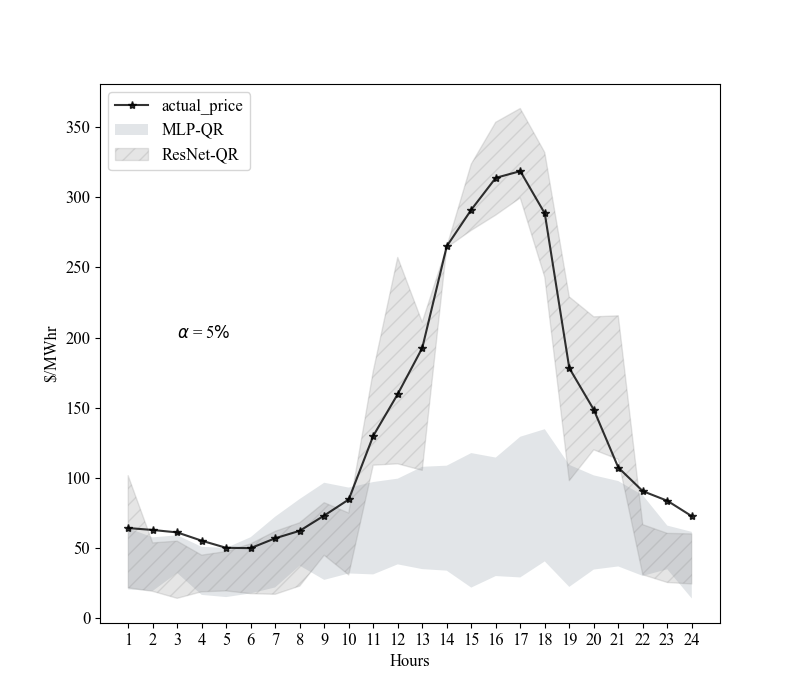
\includegraphics[width=12cm]{Task_9-compare_between_non-spike_and_spike}
      \caption{The results of MLP (non-spike price detection) model and ResNet (spike price prediction) model with quantile regression method on confidence level ($\alpha$ = 5$\%$ on Task 9)}
      \label{Fig:compare_spike_and_non_spike_model}
    \end{figure}

    Figure~\ref{Fig:all_task_QR_005} presents overall results of interval electricity price prediction of ResNet-QR model with 5$\%$ confidence level.
    In task 4, 5, 6, 11, 12, 13 and 14, there is no number of spike price in the system.
    The proposed ResNet-QR can predict lower and upper electricity price bound and cover the fluctuated real prices in these task.
    Furthermore, the proposed ResNet-QR model has capability of interval prediction of spike price occured in task 7, 8, 9 and 10.

    \begin{figure}[H]
      \centering
      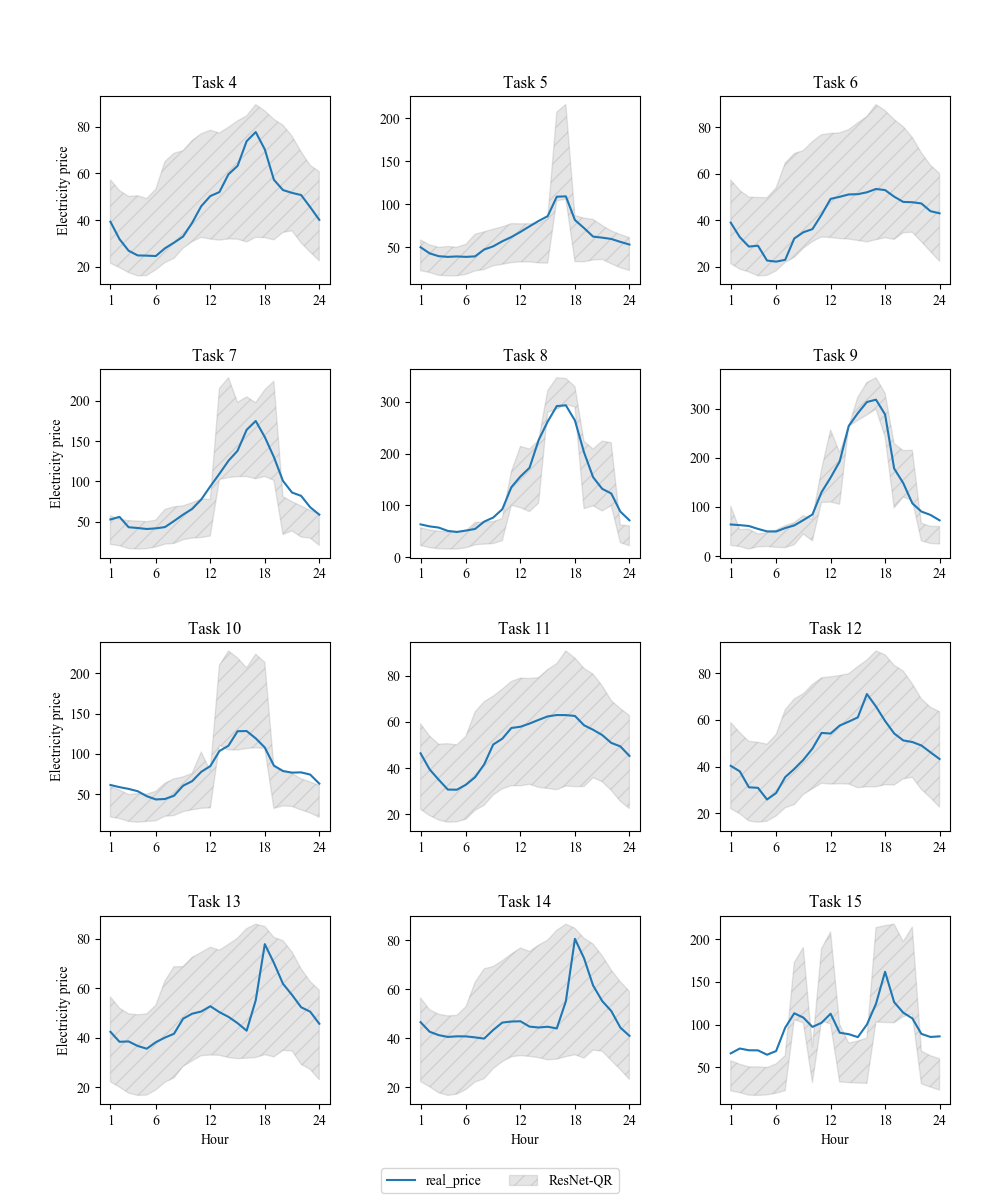
\includegraphics[width=15cm]{All_task_with_spike_price_QR_005}
      \caption{The results of ResNet-QR with 5$\%$ confidence level in task 4-15.}
      \label{Fig:all_task_QR_005}
    \end{figure}

    Second, we will discuss more on the effect of confidence levels ($\alpha$) to reliability aspect of proposed model here.
    All CWC values are analysed using distribution characteristic in each model at differenced confidence level (5$\%$, 10$\%$, 15$\%$, 20$\%$ and 25$\%$).
    The Figure~\ref{Fig:CWC} illustrateds all CWC value where bold line represents average CWC values, of all task, of particular model and confidence level.
    The boxes contain 50$\%$ of CWC values.
    The top and buttom wiskers show highest and lowest CWC values in each box.
    Since CWC value represents both coverage probility and width perspective, the lower CWC value represents higher reliability.
    The Figure~\ref{Fig:CWC} shows that while increasing confidence level, the models could perform better in CWC perspective.
    The averaged CWC value could drop below 15 while increasing confidence level up to 15 $\%$ for ResNet models.
    Moreover, quantile regression method provides higher reliabaility aspect than mean-variance method as seen in Figure~\ref{Fig:CWC}.

    \begin{figure}[H]
      \centering
      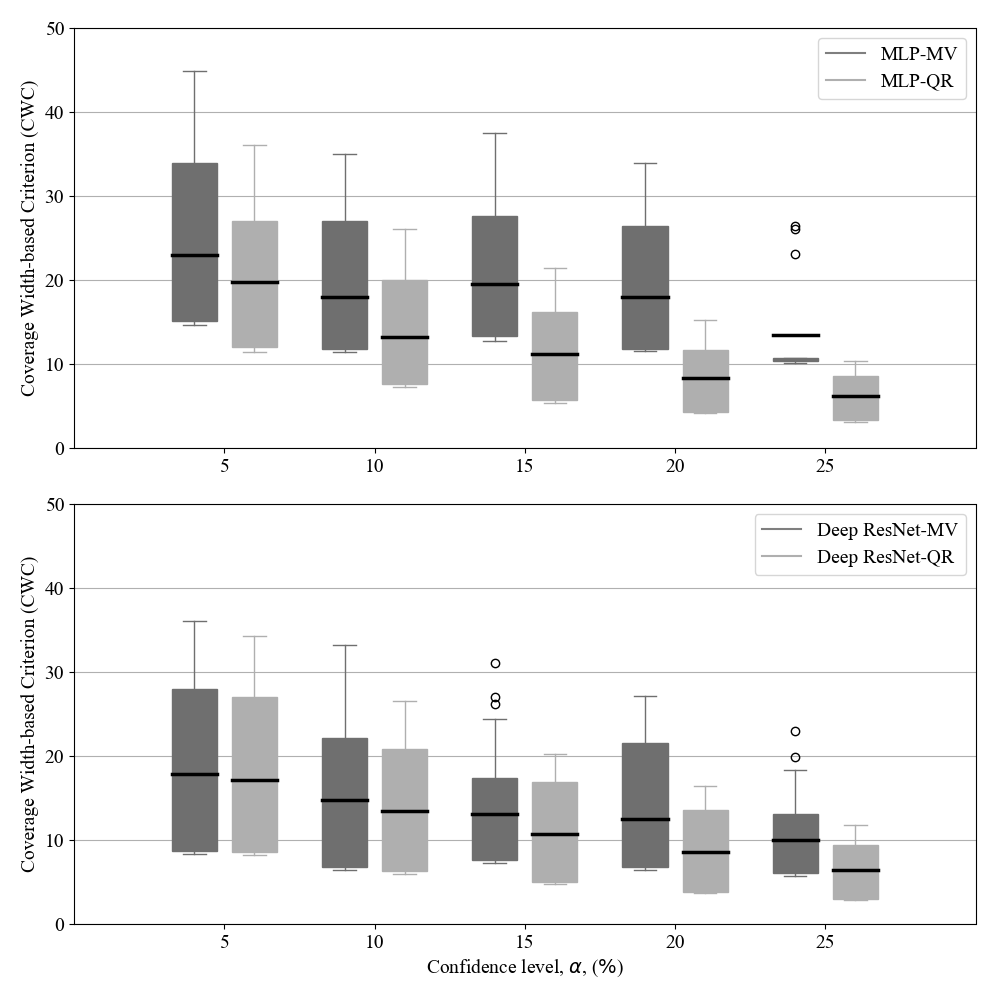
\includegraphics[width=12cm]{boxcompare_MV-QR}
      \caption{The results of reliability aspect are represented in CWC values (upper) MLP model, (lower) ResNet model.}
      \label{Fig:CWC}
    \end{figure}

    In summary, we've already considered both accuracy and reliability aspects of proposed ResNet models through pinball losses score and CWC values, respectively.
    The MLP models has low performance on task 8 and 9 where spike prices occures in the tasks.
    In addition, the MLP models could not predict the range of electricity price during high forecasted system and zonal load.
    On the other hand, ResNet model can covered forecast interval of electricity price in mostly tasks where MLP could not.
    Lastly, quantile regression method performs similar pinball loss score results comparing to mean and variance estimation method in accuracy aspect.
    However, quantile regression method provider better CWC values.
    Consequently, the proposed ResNet with quantile regression could perform best in both accuracy and reliability aspect of forecasting model.

  \section{Conclusions}
    This paper proposes a novel application of Residual Neural Network (ResNet) based approach to probabilistic electricity price forecasting in term of quaintile regression and mean-varience estimation as lower and upper bound construction.
    The proposed models are demonstrated with GEFCom2014's electricity price forcasting tasks. The results of proposed and benchmark models are evaluated in accuracy and reliability point of view through pinball loss function and coveraged width-based criterion (CWC).

    The two significatant observation results were:
    (i) the electricity price forecasting model, the proposed ResNet model, with high and spike price prediciton capability can performe better than simply plain model, MLP model,
    (ii) the lower and upper bound of interval prediction using the asymmetrical model (quantile regression) could perform better than the symmetrical model (mean and varience estimation) since it could reduce width of interval prediction.
    To improve the quality of the forecasting model in the future studies, the proposed ResNet model should cooperate with other LUBE method.
    The other LUBE has its characteristics which may provide better CWC values.
    The second way to improve the performance of the proposed ResNet forecasting model is to increase the layers with in the model.
    The fined tuning forecasting deep ResNet model may performe excellent job on electricity price forecasting task.

  \section*{References}
  \bibliography{mybibfile}
\end{document}
